\documentclass[9pt,xcolor={dvipsnames}]{beamer}

\usetheme{Rochester}
\usecolortheme{beaver}

\setbeamersize{text margin left=5mm,text margin right=5mm}

\usepackage{minted}
\usepackage[utf8]{inputenc}
\usepackage[english]{babel}
\usepackage{latexsym}
\usepackage{amssymb}
\usepackage{amsmath}
\usepackage{amsthm}
\usepackage{thm-restate}
\usepackage{mathpartir}
\usepackage{epsfig}
\usepackage{stmaryrd}
\usepackage{color}
\usepackage[dvipsnames]{xcolor}
\usepackage{epstopdf}
\usepackage{microtype}
\usepackage{hyperref}
\usepackage[en-GB]{datetime2}
\DTMlangsetup[en-GB]{showdayofmonth=false}
\usepackage{lipsum}
\usepackage{caption}
\usepackage{subcaption}
\usepackage{pftools}
\usepackage{iris}
\usepackage{heaplang}
\usepackage{tikz}
\usetikzlibrary{calc,shapes.multipart,chains,arrows,scopes,decorations.markings}
\usepackage{xspace}
\usepackage{lineno}
\usepackage{booktabs}
\usepackage{tabularx}
\usepackage{multirow}
\usepackage{adjustbox}
\usepackage{csquotes}
\usepackage{natbib}
\usepackage{mathpartir}

\renewcommand*\sfdefault{lmss}
\renewcommand*\ttdefault{txtt}
\definecolor{codebg}{HTML}{f0f0f0}
\definecolor{ExampleColour}{RGB}{0, 128, 0}

\newcommand{\isLock}{\operatorname{isLock}}
\newcommand{\locked}{\operatorname{locked}}
\newcommand{\issued}{\operatorname{issued}}
\newcommand{\newLock}{\operatorname{newLock}}
\newcommand{\acquire}{\operatorname{acquire}}
\newcommand{\wait}{\operatorname{wait}}
\newcommand{\release}{\operatorname{release}}
\newcommand{\lockInv}{\operatorname{lockInv}}
\newcommand{\initialise}{\operatorname{initialize}}
\newcommand{\enqueue}{\operatorname{enqueue}}
\newcommand{\dequeue}{\operatorname{dequeue}}
\newcommand{\unwrap}{\operatorname{unwrap}}
\newcommand{\enqdeq}{\operatorname{enqdeq}}
\newcommand{\queueAdd}{\operatorname{queueAdd}}
\newcommand{\parcomp}{\ensuremath{\mathbin{||}}}

\newcommand{\msq}{M\&S Queue}
\newcommand{\tlmsq}{Two-Lock \msq{}}
\newcommand{\lfmsq}{Lock-Free \msq{}}

\newcommand{\isqueue}{\operatorname{isQueue}}
\newcommand{\isqueueseq}{\operatorname{isQueue_{S}}}
\newcommand{\isqueueconc}{\operatorname{isQueue_{C}}}
\newcommand{\TLQueueInvariantConc}{\operatorname{I_{TLC}}}
\newcommand{\TLQueueInvariantConcSimpl}{\operatorname{I^{\prime}_{TLC}}}
\newcommand{\TLQueueInvariantHocap}{\operatorname{I_{TLH}}}
\newcommand{\LFQueueInvariantHocap}{\operatorname{I_{LFH}}}
\newcommand{\SeqQgnames}{SeqQgnames}
\newcommand{\ConcQgnames}{ConcQgnames}
\newcommand{\Qgnames}{Qgnames}
\newcommand{\QueueAddInvariant}{I_{QA}}

\newcommand{\vq}{v_q}
\newcommand{\xsc}{xs}
\newcommand{\xsqueue}{xs_{\mathrm{queue}}}
\newcommand{\xsold}{xs_{\mathrm{old}}}

\newcommand{\isLLchain}{\operatorname{isLL\_chain}}
\newcommand{\isLL}{\operatorname{isLL}}
\newcommand{\AllP}{\operatorname{All}}
\newcommand{\projval}{\operatorname{projVal}}
\newcommand{\wrapsome}{\operatorname{wrapSome}}
\newcommand{\isFirst}{\operatorname{isFirst}}
\newcommand{\isLast}{\operatorname{isLast}}
\newcommand{\isSndLast}{\operatorname{isSndLast}}
\newcommand{\projqgnamesseq}{\operatorname{projQgnames_{S}}}
\newcommand{\projqgnamesconc}{\operatorname{projQgnames_{C}}}

\newcommand{\locin}{\loc_{\mathrm{in}}}
\newcommand{\locinM}[1]{\loc_{#1\_\mathrm{in}}}
\newcommand{\locout}{\loc_{\mathrm{out}}}
\newcommand{\locoutM}[1]{\loc_{#1\_\mathrm{out}}}

\newcommand{\locN}[1]{\loc_{\mathrm{#1}}}
\newcommand{\lochead}{\locN{head}}
\newcommand{\loctail}{\locN{tail}}
\newcommand{\locqueue}{\locN{queue}}

\newcommand{\nodeval}{\valB}
\newcommand{\nodevalM}[1]{\nodeval_{#1}}

\newcommand{\nIn}[1]{\operatorname{in}(#1)}
\newcommand{\nVal}[1]{\operatorname{val}(#1)}
\newcommand{\nOut}[1]{\operatorname{out}(#1)}

\newcommand{\node}{x}
\newcommand{\nodeM}[1]{\node_{#1}}
\newcommand{\nodeN}[1]{\node_{\mathrm{#1}}}
\newcommand{\nodehead}{\nodeN{head}}
\newcommand{\nodetail}{\nodeN{tail}}
\newcommand{\nodelast}{\nodeN{last}}
\newcommand{\nodenew}{\nodeN{new}}
\newcommand{\nodeheadnext}{\nodeN{head\_next}}
\newcommand{\nodetailnext}{\nodeN{tail\_next}}
\newcommand{\nodenewtail}{\nodeN{newtail}}

\newcommand{\absvalue}{\val}
\newcommand{\absvalueList}{xs_v}

\newcommand{\Hlock}{h_{\mathrm{lock}}}
\newcommand{\Tlock}{t_{\mathrm{lock}}}
\newcommand{\Hlockvar}{H\_lock}
\newcommand{\Tlockvar}{T\_lock}

\newcommand{\prophval}{\val_p}

\newcommand{\StaticState}{\textbf{Static}\xspace}
\newcommand{\EnqueueState}{\textbf{Enqueue}\xspace}
\newcommand{\DequeueState}{\textbf{Dequeue}\xspace}
\newcommand{\BothState}{\textbf{Both}\xspace}

\newcommand{\Qg}{G}
\newcommand{\Qgseq}{G_{S}}
\newcommand{\Qgconc}{G_{C}}
\newcommand{\Qghocap}{G_{H}}
\newcommand{\QAg}{Ga}

\newcommand{\ghlock}{\gname_{\mathrm{Hlock}}}
\newcommand{\gtlock}{\gname_{\mathrm{Tlock}}}
\newcommand{\gabst}{\gname_{\mathrm{Abst}}}
\newcommand{\ghead}{\gname_{\mathrm{Head}}}
\newcommand{\gtail}{\gname_{\mathrm{Tail}}}
\newcommand{\glast}{\gname_{\mathrm{Last}}}

\newcommand{\Token}[1]{\operatorname{Token}(#1)}
\newcommand{\TokE}[1]{\operatorname{TokE} ~ #1}
\newcommand{\TokEQg}{\TokE{\Qg}}
\newcommand{\TokNE}[1]{\operatorname{TokNE} ~ #1}
\newcommand{\TokNEQg}{\TokNE{\Qg}}
\newcommand{\TokD}[1]{\operatorname{TokD} ~ #1}
\newcommand{\TokDQg}{\TokD{\Qg}}
\newcommand{\TokND}[1]{\operatorname{TokND} ~ #1}
\newcommand{\TokNDQg}{\TokND{\Qg}}
\newcommand{\TokBefore}[1]{\operatorname{TokBefore} ~ #1}
\newcommand{\TokBeforeQg}{\TokBefore{\Qg}}
\newcommand{\TokAfter}[1]{\operatorname{TokAfter} ~ #1}
\newcommand{\TokAfterQg}{\TokAfter{\Qg}}
\newcommand{\TokUpdated}[1]{\operatorname{TokUpdated} ~ #1}
\newcommand{\TokUpdatedQg}{\TokUpdated{\Qg}}
\newcommand{\TokDo}[1]{\operatorname{TokD1} ~ #1}
\newcommand{\TokDoQAg}{\TokDo{\QAg}}
\newcommand{\TokDt}[1]{\operatorname{TokD2} ~ #1}
\newcommand{\TokDtQAg}{\TokDt{\QAg}}
\newcommand{\TokA}[1]{\operatorname{TokA} ~ #1}
\newcommand{\TokAQAg}{\TokA{\QAg}}
\newcommand{\TokB}[1]{\operatorname{TokB} ~ #1}
\newcommand{\TokBQAg}{\TokB{\QAg}}

\newcommand\catenate{\mathbin{\text{\ttfamily\upshape ++}}}

\newcommand{\BB}{\ensuremath{\mathbb{B}}}
\newcommand{\Cc}{\ensuremath{\mathbf{C}}}
\newcommand{\El}{\ensuremath{\mathcal{E}}}
\newcommand{\Sl}{\ensuremath{\mathcal{S}}}
\newcommand{\Ul}{\ensuremath{\mathcal{U}}}
\newcommand{\Dl}{\ensuremath{\mathcal{D}}}
\newcommand{\Fl}{\ensuremath{\mathcal{F}}}
\newcommand{\Pl}{\ensuremath{\mathcal{P}}}
\newcommand{\Tl}{\ensuremath{\mathcal{T}}}
\newcommand{\CC}{\ensuremath{\mathbb{C}}}
\newcommand{\KK}{\ensuremath{\mathbb{K}}}
\newcommand{\PP}{\ensuremath{\mathbb{P}}}
\newcommand{\VV}{\ensuremath{\mathbb{V}}}
\newcommand{\UU}{\ensuremath{\mathbb{U}}}
\newcommand{\DD}{\ensuremath{\mathbb{D}}}
\newcommand{\Ml}{\ensuremath{\mathcal{M}}}
\newcommand{\Vl}{\ensuremath{\mathcal{V}}}
\newcommand{\Il}{\ensuremath{\mathcal{I}}}
\newcommand{\Cl}{\ensuremath{\mathcal{C}}}
\newcommand{\Bl}{\ensuremath{\mathcal{B}}}
\newcommand{\Al}{\ensuremath{\mathcal{A}}}
\newcommand{\Gl}{\ensuremath{\mathcal{G}}}
\newcommand{\Nl}{\ensuremath{\mathcal{N}}}
\newcommand{\AAA}{\ensuremath{\mathbb{A}}}
\newcommand{\EE}{\ensuremath{\mathbb{E}}}

\newcommand{\isNode}[1]{\nIn{#1} \mapsto^{\persistently} (\nVal{#1}, \nOut{#1})}

\newcommand{\abstractstatefrac}[3]{#1 \Mapsto\kern-0.5ex\tfrac{1}{#2} #3}
\newcommand{\abstractstate}[3]{#1 \Mapsto^{#2}_{\circ} #3}
\newcommand{\abstractstatefullfrag}[2]{#1 \Mapsto_{\circ} #2}
\newcommand{\abstractstateauth}[2]{#1 \Mapsto_{\bullet} #2}

\newcommand{\reach}[2]{#1 \leadsto #2}
\newcommand{\ar}[2]{#1 \dashrightarrow #2}
\newcommand{\ap}[2]{#1 \rightarrowtail #2}

%%%%%%%%%%%%%%%%%%%%%%%%%%%%%%%%%%%%%%%%%%%%%%%%%%%%%%%%%%%%%%%%%%%%%%%
% Specifications

% ------ Sequential Specification ------
% Initialise

\newcommand{\seqspecinitHTGen}[2]{\hoare{\TRUE}{\initialise \ \TT}{#1 . \Exists #2. \isqueueseq(#1, [], #2)}}

\newcommand{\seqspecinitGen}[2]{\seqspecinitHTGen{#1}{#2}}

\newcommand{\seqspecinit}{\seqspecinitGen{\vq}{\Qg}}

% Enqueue
\newcommand{\seqspecenqHT}[4]{\hoare{\isqueueseq(#1, #3, #4)}{\enqueue \ #1 \ #2}{\valB . \isqueueseq(#1, (#2 :: #3), #4)}}

\newcommand{\seqspecenqGen}[4]{\All #1, #2, #3, #4. \seqspecenqHT{#1}{#2}{#3}{#4}}

\newcommand{\seqspecenq}{\seqspecenqGen{\vq}{\absvalue}{\absvalueList}{\Qg}}

% Dequeue
\newcommand{\seqspecdeqHT}[3]{\hoareV[t]{\isqueueseq(#1, #2, #3)}{\dequeue \ #1}{\nodeval . \begin{array}{l}(#2 = [] \star{} \nodeval = \None \star{} \isqueueseq(#1, #2, #3)) \lor{}\\ (\Exists \absvalue, #2' . #2 = #2' \catenate [\absvalue] \star{} \nodeval = \Some \absvalue \star{} \isqueueseq(#1, #2', #3)) \end{array}}}

\newcommand{\seqspecdeqGen}[3]{\All #1, #2, #3. \seqspecdeqHT{#1}{#2}{#3}}

\newcommand{\seqspecdeq}{\seqspecdeqGen{\vq}{\absvalueList}{\Qg}}


% ------ Concurrent Specification ------
% Initialise
\newcommand{\concspecinitHTGen}[3]{\hoare{\TRUE}{\initialise \ \TT}{#2 . \Exists #3. \isqueueconc(#1, #2, #3)}}

\newcommand{\concspecinitGen}[3]{\concspecinitHTGen{#1}{#2}{#3}}

\newcommand{\concspecinit}[1]{\concspecinitGen{#1}{\vq}{\Qg}}

% Enqueue
\newcommand{\concspecenqHT}[4]{\hoare{\isqueueconc(#1, #2, #4) \star{} #1(#3)}{\enqueue \ #2 \ #3}{\valB . \TRUE}}

\newcommand{\concspecenqGen}[4]{\All #2, #3, #4. \concspecenqHT{#1}{#2}{#3}{#4}}

\newcommand{\concspecenq}[1]{\concspecenqGen{#1}{\vq}{\absvalue}{\Qg}}

% Dequeue
\newcommand{\concspecdeqHT}[3]{\hoare{\isqueueconc(#1, #2, #3)}{\dequeue \ #2}{\nodeval . \nodeval = \None \lor{} (\Exists \absvalue . \nodeval = \Some \absvalue \star{} #1(\absvalue))}}

\newcommand{\concspecdeqGen}[3]{\All #2, #3. \concspecdeqHT{#1}{#2}{#3}}

\newcommand{\concspecdeq}[1]{\concspecdeqGen{#1}{\vq}{\Qg}}


% ------ HOCAP-style Specification ------
% Initialise
\newcommand{\hocapspecinitHTGen}[2]{\hoare{\TRUE}{\initialise \ \TT}{#1 . \Exists #2 . \isqueue(#1, #2) \star{} \abstractstatefullfrag{#2.\gabst}{[]}}}

\newcommand{\hocapspecinitGen}[2]{\hocapspecinitHTGen{#1}{#2}}

\newcommand{\hocapspecinit}{\hocapspecinitGen{\vq}{\Qg}}

% Enqueue
\newcommand{\hocapspecenqVS}[5]{\abstractstateauth{#2.\gabst}{#5} \star{} #3 \vs[\mask\setminus\Nl.i^\uparrow] \later \abstractstateauth{#2.\gabst}{(#1 :: #5)} \star{} #4}

\newcommand{\hocapspecenqHT}[5]{\hoare{\isqueue(#1, #3) \star{} #4}{\enqueue \ #1 \ #2}{\valB . #5}}

\newcommand{\hocapspecenqGen}[6]{\All #1, #2, #3, #4, #5.
\begin{array}[t]{l}
\left(\All #6 . \hocapspecenqVS{#2}{#3}{#4}{#5}{#6} \right)
\wand\\
\hocapspecenqHT{#1}{#2}{#3}{#4}{#5}
\end{array}}

\newcommand{\hocapspecenq}{\hocapspecenqGen{\vq}{\absvalue}{\Qg}{P}{Q}{\absvalueList}}

% Dequeue
\newcommand{\hocapspecdeqVSGen}[6]{
  \abstractstateauth{#1.\gabst}{#4} \star{} #2 \vs[\mask\setminus\Nl.i^\uparrow] \later
  \left(
    \begin{array}{l}
      (#4 = [] \star{} \abstractstateauth{#1.\gabst}{#4} \star{} #3(\None))\\
      \lor{}
      \left(
        \begin{array}{l}
          \Exists #5, #6 . #4 = #6 \catenate [#5] \star{}\\
          \abstractstateauth{#1.\gabst}{#6} \star{} #3(\Some{#5})
        \end{array}
        \right)
    \end{array}
  \right)
}
\newcommand{\hocapspecdeqVS}[4]{\hocapspecdeqVSGen{#1}{#2}{#3}{#4}{\absvalue}{#4'}}

\newcommand{\hocapspecdeqHT}[4]{\hoare{\isqueue(#1, #2) \star{} #3}{\dequeue \ #1}{\nodeval . #4(\nodeval)}}

\newcommand{\hocapspecdeqGen}[5]{\begin{array}[t]{l}
  \All #1, #2, #3, #4.\\
  \begin{array}[t]{l}
  \quad\left(\All #5 . \hocapspecdeqVS{#2}{#3}{#4}{#5} \right) \wand\\
  \quad\hocapspecdeqHT{#1}{#2}{#3}{#4}
  \end{array}
\end{array}}

\newcommand{\hocapspecdeq}{\hocapspecdeqGen{\vq}{\Qg}{P}{Q}{\absvalueList}}


%%%%%%%%%%%%%%%%%%%%%%%%%%%%%%%%%%%%%%%%%%%%%%%%%%%%%%%%%%%%%%%%%%%%%%%
% Inferences Rules
% From https://github.com/logsem/iris-lecture-notes

%% Macros for constructing iterated inference rules with similar labels
% Constructs a rule with name #2, label #3 (with postfix #1; default empty),
% hypotheses #4 and conclusion #5
% ex: \rulegenhref[-app]{$\ast$-weak}{star-weak}{ }{P_1 \ast P_2 \proves P_1}
\newcommand{\rulegenhref}[5][]{\inferhref{#2}{#3#1}{#4}{#5}}
% Variant for constructing bi-inference rules
\newcommand{\rulegenhrefb}[5][]{\inferhrefB{#2}{#3#1}{#4}{#5}}
% Variant where name and label coincide
\newcommand{\rulegen}[4][]{\rulegenhref[#1]{#2}{#2}{#3}{#4}}
% Variant of bi-inference where name and label coincide
\newcommand{\rulegenb}[4][]{\rulegenhrefb[#1]{#2}{#2}{#3}{#4}}

\newcommand{\logicstarweakrule}[1][]
{ \rulegenhref[#1]{$\ast$-weak}{star-weak}
  { }
  {P_1 \ast P_2 \proves P_1}}

\newcommand{\logicstarassocrule}[1][]
{ \rulegenhref[#1]{$\ast$-assoc}{star-assoc}
  { }
  {P_1 \ast (P_2 \ast P_3) \provesIff (P_1 \ast P_2) \ast P_3}}

\newcommand{\logicstarcommrule}[1][]
{ \rulegenhref[#1]{$\ast$-comm}{star-comm}
  { }
  {P_1 \ast P_2 \provesIff P_2 \ast P_1}}

\newcommand{\logicstarintrorule}[1][]
{ \rulegenhref[#1]{$\ast$I}{star-I}
  {P_1 \proves Q_1 \and P_2 \proves Q_2 }
  {P_1 \ast P_2 \proves Q_1 \ast Q_2 }}

\newcommand{\logicwandintrorule}[1][]
{ \rulegenhref[#1]{$\wand$I}{wand-I}
  {R \ast \prop \proves \propB}
  {R \proves \prop \wand \propB}}

\newcommand{\logicwandelimrule}[1][]
{ \rulegenhref[#1]{$\wand$E}{wand-E}
  {R_1 \proves \prop \wand \propB \and R_2 \proves \prop}
  {R_1 \ast R_2 \proves \propB}}

\newcommand{\persduprule}[1][]
{ \rulegen[#1]{persistently-dup}
  {}{\persistently P \provesIff \persistently P \ast P}}

\newcommand{\persintrorule}[1][]
{ \rulegen[#1]{persistently-intro}
  {\persistently P \proves Q}{\persistently P \proves \persistently Q}}

\newcommand{\perskeeprule}[1][]
{ \rulegen[#1]{persistently-keep}
  {P \proves \persistently Q}{P \proves \persistently Q \ast P}}

\newcommand{\pershtrule}[1][]
{ \rulegen[#1]{persistently-Ht}{}{\hoare{P}{e}{\Phi} \provesIff \persistently \hoare{P}{e}{\Phi}}}

\newcommand{\lobrule}[1][]
{ \rulegenhref[#1]{L{\"o}b}{Loeb}
  {Q \land \later\prop \proves \prop}
  {Q \proves \prop}}

\newcommand{\latermonorule}[1][]
{ \rulegenhref[#1]{later-mono}{Later-Mono}
  {Q \proves \prop}
  {\later Q \proves \later\prop}}

\newcommand{\laterweakrule}[1][]
{ \rulegenhref[#1]{later-weak}{Later-weak}
  {Q \proves \prop}
  {Q \proves \later{\prop}}}

\newcommand{\htframe}[1][]
{ \rulegen[#1]{Ht-frame}
  {S \proves \hoare{P}{e}{v.Q}}
  {S \proves \hoare{P \ast R}{e}{v.Q \ast R}}}

\newcommand{\htret}[1][]
{ \rulegen[#1]{Ht-ret}
  {w \text{ is a value }}
  {S \proves \hoare{\TRUE}{\valB}{v. v = \valB}}}

\newcommand{\htbind}[1][]
{\rulegen[#1]{Ht-bind}
  { \text{$\lctx$ is an eval. context} \and
    S \proves \hoare{\prop}{\expr}{\Ret\val. \propB} \and
    S \proves \All \val. \hoare{\propB}{\lctx[\val]}{\Ret\valB.\propC}}
  { S \proves \hoare{\prop}{\lctx[\expr]}{\Ret\valB.\propC}}}

\newcommand{\htloadgen}[2][]
{ \rulegen[#1]{Ht-load}
  { }
  { S \proves \hoare{#2 \ell \pointsto u}{\deref \ell}{v . v = u \land \ell \pointsto u}}}

\newcommand{\htloadtemp}[1][]
{ \htloadgen[-temp#1]{ }}

\newcommand{\htalloc}[1][]
{ \rulegen[#1]{Ht-alloc}
  { }
  { S \proves \hoare{\TRUE}{\Ref(u)}{v . \Exists \ell . v = \ell\land \ell \pointsto u}}}

\newcommand{\htstoregen}[2][]
{ \rulegen[#1]{Ht-store}
  { }
  { S \proves \hoare{#2 \ell \pointsto -}{\ell \gets w }{v . v = \TT \land \ell \pointsto w}}}

\newcommand{\htstoretemp}[1][]
{\htstoregen[-temp#1]{ }}


%% Generic command for constructing variations of the consequence rule
\newcommand{\htcsq}[1][]
{ \rulegen[#1]{Ht-csq}
  { S \text{ persistent } \and
  S \proves \prop \Rightarrow{} \prop' \and
  S \proves \hoare{\prop'}{\expr}{\Ret\val.\propB'} \and
  S \proves \All u. \propB'[u/v] \Rightarrow{} \propB[u/v]}
  {S \proves \hoare{\prop}{\expr}{\Ret\val.\propB}}}

\newcommand{\htcsqvsrule}[1][]
{ \rulegen[#1]{Ht-csq-vs}
  { S \proves \prop \vs \prop' \and
    S \proves \hoare{\prop'}{\expr}{\Ret\val.\propB'} \and
    S \proves \All u. \propB'[u/v] \vs \propB[u/v]}
  {S \proves \hoare{\prop}{\expr}{\Ret\val.\propB}}}

\newcommand{\htbetagen}[4][]
{ \rulegen[#1]{Ht-beta#1}
  {S \proves \hoare{P}{e\left[v/x\right]}{u.Q}[#3]}
  {S \proves \hoare{#2 P}{(\lambda x . e) v}{u.Q}[#3]}}

\newcommand{\htbeta}[1][]{\htbetagen[#1]{ }{ }}

\newcommand{\htbetalater}[1][]{\htbetagen[-later#1]{\later}{}}

\newcommand{\htloadlaterrule}[1][]{\htloadgen[#1]{\later}}

\newcommand{\htstorelaterrule}[1][]{\htstoregen[#1]{\later}}

\newcommand{\Htpar}[1][]
{ \rulegen[#1]{Ht-par}
    {S \proves \hoare{P_1}{e_1}{v.Q_1} \and S \proves \hoare{P_2}{e_2}{v.Q_2}}
    {S \proves \hoare{P_1 \ast P_2}{e_1 \parcomp e_2}{v.\Exists v_1 v_2.v = (v_1,v_2) \ast Q_1[v_1/v] \ast Q_2[v_2/v]}}}

\newcommand{\fpurule}[1][]
{ \rulegen[#1]{frame-preserving-update}
  {}{a \mupd b \iff \forall x \in \Ml, a \cdot x \in \Vl \implies b \cdot x \in \Vl.}}

\newcommand{\updmonorule}[1][]
{\rulegen[#1]{upd-mono}
  {P \proves Q}
  {\pvs P \proves \pvs Q}}

\newcommand{\updintrorule}[1][]
{\rulegen[#1]{upd-intro}{ }
  {P \proves \pvs P}}

\newcommand{\updidemprule}[1][]
{\rulegen[#1]{upd-idemp}
  { }
  {\pvs \pvs P \proves \pvs P}}

\newcommand{\updframerule}[1][]
{\rulegen[#1]{upd-frame}
  { }
  {P \ast \pvs Q \proves \pvs (P \ast Q)}}

\newcommand{\ghostallocrule}[1][]
{\rulegen[#1]{Ghost-alloc}
  {a \in \Vl}
  {\TRUE \proves \pvs \Exists \gamma . \ownGhost{\gamma}{a}}}

\newcommand{\ghostupdaterule}[1][]
{\rulegen[#1]{Ghost-update}
  {a \mupd b}
  { \ownGhost{\gamma}{a} \proves \pvs \ownGhost{\gamma}{b}}}

\newcommand{\ownoprule}[1][]
{ \rulegen[#1]{Own-op}
  { }
  {\ownGhost{\gamma}{a} \ast \ownGhost{\gamma}{b} \provesIff \ownGhost{\gamma}{a \cdot b}}}

\newcommand{\ownvalidrule}[1][]
{ \rulegen[#1]{Own-valid}
  { }
  {\ownGhost{\gamma}{a} \proves a \in \Vl}}

\newcommand{\invalloc}
{ \rulegen[]{Inv-alloc}
  {}
  {\later P \proves \pvs[\emptyset] \knowInv{\Nl}{P}}}

\newcommand{\wpinvopen}[1][]
{ \rulegen[#1]{wp-inv-open-namespace}
  {e \text{ is an atomic expression } \and \Nl^\uparrow \subseteq \mask}
  {\knowInv{\Nl}{P} \ast \left(\later P \wand \wpre{e}[\mask\setminus\Nl^\uparrow]{v.\later P \ast \Phi(v)}\right)
    \proves{}
    \wpre{e}[\mask]{\Phi}}}

%%%%%%%%%%%%%%%%%%%%%%%%%%%%%%%%%%%%%%%%%%%%%%%%%%%%%%%%%%%%%%%%%%%%%%%

\AtBeginSection[]{
  \begin{frame}
  \vfill
  \centering
  \begin{beamercolorbox}[sep=8pt,center,shadow=true,rounded=true]{title}
    \usebeamerfont{title}\insertsectionhead\par%
  \end{beamercolorbox}
  \vfill
  \end{frame}
}


\addtobeamertemplate{navigation symbols}{}{%
    \usebeamerfont{footline}%
    \usebeamercolor[fg]{footline}%
    \hspace{1em}%
    \insertframenumber/\inserttotalframenumber
}

% Colour for connectives
\let\oldlor\lor
\renewcommand{\lor}{\begingroup \color{red} \oldlor \endgroup}

\let\oldland\land
\renewcommand{\land}{\begingroup \color{Emerald} \oldland \endgroup}

\let\oldstar\star
\renewcommand{\star}{\begingroup \color{Emerald} \oldstar \endgroup}

%%%%%%%%%%%%%%%%%%%%%%%%%%%%%%%%%%%%%%%%%%%%%%%%%%%%%%%%%%%%%%%%%%%%%%%

\title{Master's Thesis Exam\\
Verification of the Blocking and Non-Blocking Michael-Scott Queue Algorithms}
\author{
  Mathias Pedersen, 201808137 \texorpdfstring{\\}{with}
  {\small Advisor: Amin Timany}
}
\institute{Aarhus University}
\date{\today}
\titlegraphic {
\begin{tikzpicture}[overlay,remember picture]
\node[right=0.3cm] at (current page.210){
    
\includegraphics[scale=0.7]{../thesis/logo.eps}
};
\end{tikzpicture}
}

%%%%%%%%%%%%%%%%%%%%%%%%%%%%%%%%%%%%%%%%%%%%%%%%%%%%%%%%%%%%%%%%%%%%%%%

\newcommand{\todo}[1]{{\color[rgb]{.5,0,0}\textbf{$\blacktriangleright$#1$\blacktriangleleft$}}}

\begin{document}

\frame{\titlepage}

%%%%%%%%%%%%%%%%%%%%%%%%%%%%%%%%%%%%%%%%%%%%%%%%%%%%%%%%%%%%%%%%%%%%%%%

\begin{frame}{Overview of the Project and Contributions}
  \begin{itemize}
    \item Initial \textcolor{blue}{goal} was to prove \textcolor{blue}{safety} of the two \textcolor{blue}{\msq{}s}
    \item The project later \textcolor{Turquoise}{generalised} the results to apply to \textcolor{blue}{queues in general}
    \pause
    \item In particular, three different \textcolor{blue}{specifications for queues} were given
    \begin{itemize}
      \item \textcolor{orange}{Sequential} specification
        \begin{itemize}
          \item Useful for sequential clients
        \end{itemize}
      \item \textcolor{orange}{Concurrent} specification
        \begin{itemize}
          \item Proves \textcolor{blue}{safety of concurrent queues}
          \item Useful for \textit{some} concurrent clients
          \item \textcolor{red}{Doesn't track} queue contents
        \end{itemize}
      \item \textcolor{orange}{HOCAP-style} specification
        \begin{itemize}
          \item Stronger specification, useful for more \textcolor{blue}{complex clients}
          \item \textcolor{blue}{Tracks} queue contents
          \item Demonstrated with a PoC queue client, QueueAdd
        \end{itemize}
    \end{itemize}
    \pause
    \item It was demonstrated that the HOCAP-style specification \textcolor{blue}{derives the sequential and concurrent specifications}
    \pause
    \item \textcolor{ExampleColour}{Implementations} of the \msq{}s in \textcolor{blue}{\heaplang{}} were proven to meet the three \textcolor{blue}{specifications}
      \begin{itemize}
        \item In particular, both version are \textcolor{blue}{safe}
      \end{itemize}
    \pause
    \item All proofs have been \textcolor{blue}{mechanised} in the \textcolor[RGB]{199,154,115}{Coq} \textcolor[RGB]{222,196,152}{proof assistant}
  \end{itemize}
\end{frame}
%%%%%%%%%%%%%%%%%%%%%%%%%%%%%%%%%%%%%%%%%%%%%%%%%%%%%%%%%%%%%%%%%%%%%%%

% Outline
\begin{frame}{Outline}
  \tableofcontents
\end{frame}

%%%%%%%%%%%%%%%%%%%%%%%%%%%%%%%%%%%%%%%%%%%%%%%%%%%%%%%%%%%%%%%%%%%%%%%

\section{Queue Specifications (HOCAP)}

%=====================================================================
\begin{frame}{Specifications for Queues}
  \begin{block}{Assumptions on Queues}
    \begin{itemize}
      \item Queues consists of \textcolor{Brown}{$\initialise$}, \textcolor{Brown}{$\enqueue$}, and \textcolor{Brown}{$\dequeue$}
      \item \textcolor{Brown}{$\initialise$} creates an \textcolor{blue}{empty queue}: $[]$
      \item \textcolor{Brown}{$\enqueue$} adds a value, $\absvalue$, to the \textcolor{blue}{beginning of the queue} $\absvalueList$: $\absvalue :: \absvalueList$
      \item \textcolor{Brown}{$\dequeue$} depends on whether queue is empty:
        \begin{itemize}
          \item If \textcolor{blue}{non-empty}, $\absvalueList \catenate \absvalue$, remove value $\absvalue$ at \textcolor{blue}{end of queue} and return \textcolor{blue}{$\Some \absvalue$}
          \item If \textcolor{blue}{empty}, $[]$, return \textcolor{blue}{$\None$}
        \end{itemize}
    \end{itemize}
  \end{block}
  \pause
  \begin{block}{Nature of Specifications}
    \begin{itemize}
      \item Specifications written in \textcolor{blue}{Iris}, a \textcolor{blue}{higher order CSL}
      \item Expressed in terms of \textcolor{blue}{\textit{Hoare triples}}: $\hoare{P}{e}{v. \Phi ~ v}$
      \item Hoare triples prove \textcolor{blue}{partial correctness} of programs, $e$
      \item In particular: \textcolor{blue}{safety}
    \end{itemize}
  \end{block}
\end{frame}

%=====================================================================
\begin{frame}{HOCAP-style Specification - Abstract State RA}
  \begin{itemize}
    \item We will need a \textcolor{blue}{construction} to allow clients to \textcolor{blue}{track contents of queue}
    \pause
    \item Idea: have \textcolor{blue}{two} ``\textcolor{blue}{views}'' of the \textcolor{blue}{abstract state} of the queue
    \begin{columns}
      \begin{column}{0.5\textwidth}
        \begin{center}
          \textbf{Authoritative view}\\
          $\abstractstateauth{\gname}{\absvalueList}$\\
          Owned by queue\\
        \end{center}
      \end{column}
      \begin{column}{0.5\textwidth}
        \begin{center}
          \textbf{Fragmental view}\\
          $\abstractstatefullfrag{\gname}{\absvalueList}$\\
          Owned by client\\
        \end{center}
      \end{column}
    \end{columns}
    \pause
    \item Construction \textcolor{blue}{ensures}:
      \begin{itemize}
        \item \textcolor{blue}{authoritative} and \textcolor{blue}{fragmental} views always \textcolor{blue}{agree} on abstract state of queue
        \item views can only be \textcolor{blue}{updated} in \textcolor{blue}{unison}
      \end{itemize}
    \item \textcolor{blue}{Implemented} using the \textcolor{blue}{resource algebra}: $\authm(\option{(\fracm \times \agm(\List ~ \Val))})$
    \item The \textcolor{blue}{desirables} are captured by the following \textcolor{blue}{lemmas}
  \end{itemize}
  \begin{block}{Lemmas on the Abstract State RA}
    \setlength\abovedisplayskip{-8pt}
    \setlength\belowdisplayskip{2pt}
    \begin{align*}
      &\proves \pvs \Exists \gname . \abstractstateauth{\gname}{\absvalueList} \star{} \abstractstatefullfrag{\gname}{\absvalueList} & \text{(Abstract State Alloc)}\\[0.8ex]
      &\abstractstateauth{\gname}{\absvalueList'} \star{}
      \abstractstatefullfrag{\gname}{\absvalueList} \proves
      \absvalueList = \absvalueList' & \text{(Abstract State Agree)}\\[0.8ex]
      &\abstractstateauth{\gname}{\absvalueList'} \star{}
      \abstractstatefullfrag{\gname}{\absvalueList} \vs
      \abstractstateauth{\gname}{\absvalueList''} \star{}
      \abstractstatefullfrag{\gname}{\absvalueList''} & \text{(Abstract State Update)}
    \end{align*}
  \end{block}
\end{frame}

%=====================================================================
\begin{frame}{HOCAP-style Specification}
  \begin{itemize}
    \item Post-condition of \textcolor{Brown}{$\initialise$} specification gives \textcolor{blue}{fragmental view} to \textcolor{blue}{clients}
    \item Hoare triples for \textcolor{Brown}{$\enqueue$} and \textcolor{Brown}{$\dequeue$} are conditioned on \textcolor{blue}{view-shifts}
    \item Clients must show that they can \textcolor{blue}{supply} the \textcolor{blue}{fragmental view}, so that the \textcolor{blue}{abstract} (and concrete) \textcolor{blue}{state} can be \textcolor{blue}{updated}
    \item View-shifts and Hoare-triples \textcolor{blue}{parametrised} by predicates \textcolor{RubineRed}{$P$} and \textcolor{RubineRed}{$Q$}
      \begin{itemize}
        \item Client might have \textcolor{blue}{resources} that need to be \textcolor{blue}{updated} as a result of \textcolor{Brown}{$\enqueue$}/\textcolor{Brown}{$\dequeue$}
        \item \textcolor{RubineRed}{$P$} is the clients resources \textcolor{blue}{before} \textcolor{Brown}{$\enqueue$}/\textcolor{Brown}{$\dequeue$} and \textcolor{RubineRed}{$Q$} the resources \textcolor{blue}{after}
      \end{itemize}
  \end{itemize}
  \vspace{-4pt}
  \begin{definition}[HOCAP Specification]\label{QueueSpecs:spec:hocap}
    \setlength\abovedisplayskip{-8pt}
    \setlength\belowdisplayskip{2pt}
    \fontsize{7pt}{9}\selectfont
    \begin{align*}
      &\Exists \isqueue : \Val \to \Qgnames \to \Prop.\\
      &\quad\quad \All \vq, \Qg . \isqueue(\vq, \Qg) \implies \persistently \isqueue(\vq, \Qg)\\
      &\uncover<2->{\land{}\quad\hocapspecinit}\\
      &\uncover<3->{\land{}\quad\hocapspecenq}\\
      &\uncover<4->{\land{}\quad\hocapspecdeq}
    \end{align*}
  \end{definition}
\end{frame}

%%%%%%%%%%%%%%%%%%%%%%%%%%%%%%%%%%%%%%%%%%%%%%%%%%%%%%%%%%%%%%%%%%%%%%%

\section{The Two-Lock Michael-Scott Queue}

%=====================================================================
\begin{frame}[fragile]{Implementation: $\initialise$}
  \begin{itemize}
    \item The queue data structure is a \textcolor{blue}{linked list}
    \item<2-> A \textcolor{blue}{node} $\node$ in the linked list is a \textcolor{blue}{triple}, $\node = (\locin, \nodeval, \locout)$, with $\locin \mapsto (\nodeval, \locout)$
    \item<2-> We use the following \textcolor{blue}{notation} for nodes
    \begin{align*}
      &\nIn{\node} = \locin& &\nVal{\node} = \nodeval& &\nOut{\node} = \locout
    \end{align*}
    \item<3-> The \textcolor{Brown}{$\initialise$} function first creates an \textcolor{blue}{initial head node}, $\nodehead$
    \item<3-> Then, a \textcolor{blue}{lock} protecting the \textcolor{blue}{head pointer}, and a \textcolor{blue}{lock} protecting the \textcolor{blue}{tail pointer}
    \item<3-> Finally, it creates the \textcolor{blue}{head} and \textcolor{blue}{tail pointers}, $\lochead$ and $\loctail$, both \textcolor{blue}{pointing to} $\nodehead$
  \end{itemize}
  \vspace{-8pt}
  \begin{minted}[escapeinside=||, mathescape=true, bgcolor=codebg, frame=lines, fontsize=\footnotesize]{ocaml}
|$ \initialise \eqdef $|
  |$ \Let node = \Ref(\None, \Ref(\None)) in $|
  |$ \Let \Hlockvar = \newLock \TT in $|
  |$ \Let \Tlockvar = \newLock \TT in $|
  |$ \Ref((\Ref(node), \Ref(node)), (\Hlockvar, \Tlockvar)) $|
  \end{minted}
  \begin{center}
  \vspace{-6pt}
  \scalebox{0.8}{
  \begin{tikzpicture}[
    pair/.style = {
      on chain,
      rectangle split,
      rectangle split horizontal,
      rectangle split parts=2,
      draw,
      anchor=center,
      text height=1.5ex,
    },
    perspointer/.style = {
      on chain,
      rectangle,
      draw,
      anchor=center,
      text height=1.5ex,
    },
    pointer/.style = {
      rectangle,
      draw,
      anchor=center,
      text height=1.5ex,
    },
    start chain=going right,
    decoration={
      markings,
      mark=at position .5 with {\arrow{Square[length=5pt,sep=-2.5pt]}}
    },
  ]

  % Linked List
  \node (l'1) [join={by ->}, perspointer,on chain] {$\locinM{1}$};
  \node (l1pair) [join={by ->, draw=blue, postaction={decorate}}, pair,on chain] {$\None$ \nodepart{two} $\locoutM{1}$};
  \node (null) [join={by ->, draw=black}, rectangle,on chain] {$\None$};

  % Head and tail
  \node (head) [pointer, above left=of l'1] {$\lochead$};
  \node (tail) [pointer, above right=of l'1] {$\loctail$};
  \draw[->] (head) -- (l'1);
  \draw[->] (tail) -- (l'1);

  \end{tikzpicture}
  }
  \end{center}
\end{frame}

%=====================================================================
\begin{frame}[fragile]{Implementation: $\enqueue$}
  \begin{itemize}
    \item The \textcolor{Brown}{$\enqueue$} function consists of the following \textcolor{blue}{steps}
    \begin{enumerate}
      \item Create a new node, $\nodenew$, containing value to be enqueued
      \item Acquire the tail lock
      \item Add $\nodenew$ to linked list
      \item Swing tail pointer to $\nodenew$
      \item Release the tail lock
    \end{enumerate}
    \item<5-> Once a node is enqueued, its \textcolor{blue}{position} in the linked list is \textcolor{blue}{fixed}
    \item<6-> Adding and swinging \textcolor{red}{not atomic} $\rightarrow$ \textcolor{blue}{Tail} node is either \textcolor{blue}{last} or \textcolor{blue}{second last}
    \item<7-> \textcolor{Brown}{$\dequeue$} \textcolor{red}{ignores tail pointer} $\rightarrow$ \textcolor{blue}{Tail} node can \textcolor{orange}{lag} behind \textcolor{blue}{head} node
  \end{itemize}
  \vspace{-8pt}
  \begin{minted}[escapeinside=||, mathescape=true, bgcolor=codebg, frame=lines, fontsize=\footnotesize]{ocaml}
|$ \enqueue \ Q \ value \eqdef $|
  |$ \Let node = \Ref(\Some value, \Ref(\None)) in $|
  |$ \acquire (\Snd (\Snd (\deref Q))); $|
  |$ \Snd (\deref(\deref(\Snd (\Fst(\deref Q))))) \gets node; $|
  |$ \Snd (\Fst (\deref Q)) \gets node; $|
  |$ \release (\Snd (\Snd (\deref Q))) $|
  \end{minted}
  \begin{center}
  \vspace{-6pt}
  \scalebox{0.8}{
  \begin{tikzpicture}[
    pair/.style = {
      on chain,
      rectangle split,
      rectangle split horizontal,
      rectangle split parts=2,
      draw,
      anchor=center,
      text height=1.5ex,
    },
    perspointer/.style = {
      on chain,
      rectangle,
      draw,
      anchor=center,
      text height=1.5ex,
    },
    pointer/.style = {
      rectangle,
      draw,
      anchor=center,
      text height=1.5ex,
    },
    start chain=going right,
    decoration={
      markings,
      mark=at position .5 with {\arrow{Square[length=5pt,sep=-2.5pt]}}
    },
  ]

  % Linked List
  \node (l'1) [join={by ->}, perspointer,on chain] {$\locinM{1}$};
  \node (l1pair) [join={by ->, draw=blue, postaction={decorate}}, pair,on chain] {$\nodevalM{1}$ \nodepart{two} $\locoutM{1}$};
  \node (l'2) [join={by ->, draw=blue, postaction={decorate}}, perspointer,on chain] {$\locinM{2}$};
  \node (l2pair) [join={by ->, draw=blue, postaction={decorate}}, pair,on chain] {$\nodevalM{2}$ \nodepart{two} $\locoutM{2}$};
  \only<1-2>{\node (null) [join={by ->, draw=black}, rectangle,on chain] {$\None$};}
  \only<3->{\node (null) [join={by ->, dotted, draw=black}, rectangle,on chain] {\textcolor{gray}{$\None$}};}

  \only<1>{
  \node (l'3) [perspointer, above right=of l2pair, draw=none] {\phantom{$\locinM{3}$}};
  \node (l3pair) [join={by ->, draw=none}, pair,on chain, draw=none] {\phantom{$\nodevalM{3}$} \nodepart{two} \phantom{$\locoutM{3}$}};
  \node (null) [join={by ->, draw=none}, rectangle,on chain] {\phantom{$\None$}};}

  \only<2->{
  \node (l'3) [perspointer, above right=of l2pair] {$\locinM{3}$};
  \node (l3pair) [join={by ->, draw=blue, postaction={decorate}}, pair,on chain] {$\nodevalM{3}$ \nodepart{two} $\locoutM{3}$};
  \node (null) [join={by ->, draw=black}, rectangle,on chain] {$\None$};}

  \only<3->{\draw[->, draw=blue, postaction={decorate}] (l2pair) -- (l'3);}

  % Head and tail
  \node (head) [pointer, above=of l'1] {$\lochead$};
  \node (tail) [pointer, above=of l'2] {$\loctail$};
  \draw[->] (head) -- (l'1);
  \onslide<1-3>
  \draw[->] (tail) -- (l'2);
  \onslide<4->
  \draw[->, dotted] (tail) -- (l'2);
  \draw[->] (tail) -- (l'3);

  \end{tikzpicture}
  }
  \end{center}
\end{frame}

%=====================================================================
\begin{frame}[fragile]{Implementation: $\dequeue$}
  \begin{itemize}
    \item The \textcolor{Brown}{$\dequeue$} function \textcolor{blue}{checks} if queue is \textcolor{blue}{empty}
      \begin{itemize}
        \item If empty, \textcolor{blue}{return} $\None$
        \item Else, \textcolor{blue}{swing head pointer} to new head node, and \textcolor{blue}{return} its value
      \end{itemize}
    \item<3-> Dequeued node \textcolor{red}{not freed} $\rightarrow$ Linked list \textcolor{blue}{only grows}
  \end{itemize}
  \vspace{-8pt}
  \begin{minted}[escapeinside=||, mathescape=true, bgcolor=codebg, frame=lines, fontsize=\footnotesize]{ocaml}
|$ \dequeue \ Q \eqdef $|
  |$ \acquire (\Fst (\Snd (\deref Q))); $|
  |$ \Let node = \deref (\Fst (\Fst (\deref Q))) in $|
  |$ \Let new\_head = \deref (\Snd(\deref node)) in $|
  |$ \If new\_head = \None then $|
    |$ \release (\Fst (\Snd(\deref Q))); $|
    |$ \None $|
  |$ \Else $|
    |$ \Let value = \Fst (\deref new\_head) in $|
    |$ \Fst (\Fst (\deref Q)) \gets new\_head; $|
    |$ \release (\Fst (\Snd (\deref Q))); $|
    |$ value $|
  \end{minted}
  \begin{center}
  \vspace{-6pt}
  \scalebox{0.8}{
  \begin{tikzpicture}[
    pair/.style = {
      on chain,
      rectangle split,
      rectangle split horizontal,
      rectangle split parts=2,
      draw,
      anchor=center,
      text height=1.5ex,
    },
    perspointer/.style = {
      on chain,
      rectangle,
      draw,
      anchor=center,
      text height=1.5ex,
    },
    pointer/.style = {
      rectangle,
      draw,
      anchor=center,
      text height=1.5ex,
    },
    start chain=going right,
    decoration={
      markings,
      mark=at position .5 with {\arrow{Square[length=5pt,sep=-2.5pt]}}
    },
  ]

  % Linked List
  \node (l1in) [join={by ->}, perspointer,on chain] {$\locinM{1}$};
  \node (l1pair) [join={by ->, draw=blue, postaction={decorate}}, pair,on chain] {$\nodevalM{1}$ \nodepart{two} $\locoutM{1}$};
  \node (l2in) [join={by ->, draw=blue, postaction={decorate}}, perspointer,on chain] {$\locinM{2}$};
  \node (l2pair) [join={by ->, draw=blue, postaction={decorate}}, pair,on chain] {$\nodevalM{2}$ \nodepart{two} $\locoutM{2}$};
  \node (l3in) [join={by ->, draw=blue, postaction={decorate}}, perspointer,on chain] {$\locinM{3}$};
  \node (l3pair) [join={by ->, draw=blue, postaction={decorate}}, pair,on chain] {$\nodevalM{3}$ \nodepart{two} $\locoutM{3}$};
  \node (null) [join={by ->, draw=black}, rectangle,on chain] {$\None$};

  % Head and tail
  \node (head) [pointer, above=of l1pair] {$\lochead$};
  \node (tail) [pointer, above=of l3in] {$\loctail$};
  \onslide<1>{\draw[->] (head) -- (l1in);}
  \onslide<2->{\draw[->, dotted] (head) -- (l1in); \draw[->] (head) -- (l2in);}
  \draw[->] (tail) -- (l3in);

  \end{tikzpicture}
  }
  \end{center}
\end{frame}

%%%%%%%%%%%%%%%%%%%%%%%%%%%%%%%%%%%%%%%%%%%%%%%%%%%%%%%%%%%%%%%%%%%%%%%

\section{Proving that the Two-Lock Michael-Scott Queue Satisfies the HOCAP-style Specification}

%=====================================================================
\begin{frame}{The isLL Predicate}
  \begin{itemize}
    \item \textcolor{blue}{Idea}: express the \textcolor{blue}{structure} of the linked list in terms of \textcolor{blue}{points-to predicates}
    \item Also captures \textcolor{blue}{persistent} and \textcolor{blue}{non-persistent} parts of the linked list
  \end{itemize}
  \begin{definition}[Linked List Predicate]
    \setlength\abovedisplayskip{-2pt}
    \setlength\belowdisplayskip{2pt}
    \fontsize{7pt}{4pt}\selectfont
    \begin{align*}
      \isLLchain([]) \eqdef& \TRUE\\
      \isLLchain([\node]) \eqdef& \isNode{\node}\\
      \isLLchain(\node :: \node' :: \xsc) \eqdef& \isNode{\node} \star{} \nOut{\node'} \mapsto^{\persistently} \nIn{\node} \star{} \isLLchain(\node' :: \xsc)
    \end{align*}
    \hrulefill
    \setlength\abovedisplayskip{2pt}
    \begin{align*}
      \isLL([]) \eqdef& \TRUE\\
      \isLL(\node :: \xsc) \eqdef& \nOut{\node} \mapsto \None \star{} \isLLchain(\node :: \xsc)
    \end{align*}
  \end{definition}
  \begin{exampleblock}{Example}
    \setlength\abovedisplayskip{6pt}
    \setlength\belowdisplayskip{6pt}
    \fontsize{8pt}{4pt}\selectfont
    Consider the list: $\xsc = [(\locinM{3}, \nodevalM{3}, \locoutM{3}); (\locinM{2}, \nodevalM{2}, \locoutM{2});  (\locinM{1}, \nodevalM{1}, \locoutM{1})]$.
    \begin{align*}
      \isLL(\xsc) = \ \locoutM{3} \mapsto \None \ \star{} \
      &\locinM{3} \mapsto^{\persistently} (\nodevalM{3}, \locoutM{3}) \star{} \locoutM{2}	\mapsto^{\persistently} \locinM{3}\star{}\\
      &\locinM{2} \mapsto^{\persistently} (\nodevalM{2}, \locoutM{2}) \star{} \locoutM{1}\mapsto^{\persistently} \locinM{2} \star{}\\
      &\locinM{1} \mapsto^{\persistently} (\nodevalM{1}, \locoutM{1})
    \end{align*}
    \begin{center}
      \scalebox{0.8}{
      \begin{tikzpicture}[
        pair/.style = {
          on chain,
          rectangle split,
          rectangle split horizontal,
          rectangle split parts=2,
          draw,
          anchor=center,
          text height=1.5ex,
        },
        perspointer/.style = {
          on chain,
          rectangle,
          draw,
          anchor=center,
          text height=1.5ex,
        },
        pointer/.style = {
          rectangle,
          draw,
          anchor=center,
          text height=1.5ex,
        },
        start chain=going right,
        decoration={
          markings,
          mark=at position .5 with {\arrow{Square[length=5pt,sep=-2.5pt]}}
        },
      ]

      % Linked List
      \node (l1in) [join={by ->}, perspointer,on chain] {$\locinM{1}$};
      \node (l1pair) [join={by ->, draw=blue, postaction={decorate}}, pair,on chain] {$\nodevalM{1}$ \nodepart{two} $\locoutM{1}$};
      \node (l2in) [join={by ->, draw=blue, postaction={decorate}}, perspointer,on chain] {$\locinM{2}$};
      \node (l2pair) [join={by ->, draw=blue, postaction={decorate}}, pair,on chain] {$\nodevalM{2}$ \nodepart{two} $\locoutM{2}$};
      \node (l3in) [join={by ->, draw=blue, postaction={decorate}}, perspointer,on chain] {$\locinM{3}$};
      \node (l3pair) [join={by ->, draw=blue, postaction={decorate}}, pair,on chain] {$\nodevalM{3}$ \nodepart{two} $\locoutM{3}$};
      \node (null) [join={by ->, draw=black}, rectangle,on chain] {$\None$};
      \end{tikzpicture}
      }
    \end{center}
    \vspace{-2pt}
  \end{exampleblock}
\end{frame}

%=====================================================================
\begin{frame}{Invariant}
  \begin{itemize}
    \item \textcolor{blue}{Queue predicate} must be \textcolor{blue}{persistent} (according to specification)
    \item \textcolor{red}{Problem}: the queue \textcolor{blue}{relies} on \textcolor{blue}{non-persistent resources} (e.g. \textcolor{ExampleColour}{$\lochead \mapsto \nIn{\nodehead}$})
    \item \textcolor{blue}{Solution}: identify an \textcolor{blue}{\textit{invariant}} (persistent), describing the resources
  \end{itemize}
  \vspace{-6pt}
  \pause
  \hrulefill
  \vspace{-2pt}
  \begin{itemize}
    \item Contains \textcolor{blue}{abstract state} of queue -- \textcolor{blue}{existentially quantified} as it can change
    \item<3-> Defines \textcolor{blue}{structure} of the \textcolor{blue}{concrete} linked list, $\xsc$
    \item<4-> Asserts \textcolor{blue}{relation} between \textcolor{blue}{abstract state} and \textcolor{blue}{concrete state}
    \item<5-> Identifies possible \textcolor{blue}{queue states}: \StaticState, \EnqueueState, \DequeueState, and \BothState{}
      \begin{itemize}
        \item Two locks $\rightarrow$ Four queue states
        \item Invariant describes the queue resources in each state
        \item See next slide
      \end{itemize}
  \end{itemize}
  \begin{definition}[\tlmsq{} HOCAP Invariant]\label{TLMSQ:spec:hocap:invariant}
    \setlength\abovedisplayskip{0pt}
    \setlength\belowdisplayskip{2pt}
    \fontsize{7pt}{4pt}\selectfont
    \begin{align*}
      \TLQueueInvariantHocap(\lochead, \loctail, \Qg) \ \eqdef \
      &\Exists \absvalueList. \abstractstateauth{\Qg.\gabst}{\absvalueList} \star{} &&\text{\textcolor{gray}{(abstract state)}}\\
      &\uncover<3->{\Exists \xsc, \xsqueue, \xsold, \nodehead, \nodetail . &&\text{\textcolor{gray}{(concrete state)}}}\\
      &\uncover<3->{\xsc = \xsqueue \catenate [\nodehead] \catenate \xsold \star{}}\\
      &\uncover<3->{\isLL(\xsc) \star{}}\\
      &\uncover<4->{\projval(\xsqueue) = \wrapsome(\absvalueList) \star{}}\\
      &\uncover<5->{\dots}
    \end{align*}
  \end{definition}
\end{frame}

%=====================================================================
\begin{frame}{Invariant (Queue States)}
  \begin{itemize}
    \item \textcolor{blue}{Idea}: the enqueueing thread \textcolor{blue}{keeps half of tail pointer} between \textcolor{blue}{invariant openings}
    \item \textcolor{blue}{Guarantees} that the pointer is \textcolor{blue}{not updated} (full pointer needed for update)
    \item \textcolor{blue}{Similarly} for the \textcolor{blue}{dequeueing} thread
    \item $\EnqueueState$ and $\BothState$ also captures ``\textcolor{blue}{gap}'' between \textcolor{blue}{adding} $\nodenew$ and \textcolor{blue}{swinging} $\loctail$
    \item \textcolor{blue}{Tokens} used to reason about which \textcolor{blue}{state} queue is in
  \end{itemize}
  \vspace{-6pt}
  \begin{definition}[\tlmsq{} HOCAP Invariant -- continued]
    \setlength\abovedisplayskip{0pt}
    \setlength\belowdisplayskip{2pt}
    \fontsize{7pt}{4pt}\selectfont
    \begin{align*}
      \dots\\
      &\quad\lochead \mapsto \nIn{\nodehead} \star{} \loctail \mapsto \nIn{\nodetail} \star{} \isLast(\nodetail, \xsc) \star{} &&\text{\textcolor{gray}{(\StaticState)}}\\
      &\quad \TokNEQg \star{} \TokNDQg \star{} \TokUpdatedQg\\
      \lor{} &\quad\lochead \mapsto \nIn{\nodehead} \star{} \loctail \mapsto^{\frac{1}{2}} \nIn{\nodetail} \star{} &&\text{\textcolor{gray}{(\EnqueueState)}}\\
      &\quad (\isLast(\nodetail, \xsc) \star{} \TokBeforeQg \lor{} \isSndLast(\nodetail, \xsc) \star{} \TokAfterQg) \star{}\\
      &\quad \TokEQg \star{} \TokNDQg\\
      \lor{} &\quad\lochead \mapsto^{\frac{1}{2}} \nIn{\nodehead} \star{} \loctail \mapsto \nIn{\nodetail} \star{} \isLast(\nodetail, \xsc) \star{} &&\text{\textcolor{gray}{(\DequeueState)}}\\
      &\quad \TokNEQg \star{} \TokDQg \star{} \TokUpdatedQg\\
      \lor{} &\quad\lochead \mapsto^{\frac{1}{2}} \nIn{\nodehead} \star{} \loctail \mapsto^{\frac{1}{2}} \nIn{\nodetail} \star{} &&\text{\textcolor{gray}{(\BothState)}}\\
      &\quad (\isLast(\nodetail, \xsc) \star{} \TokBeforeQg \lor{} \isSndLast(\nodetail, \xsc) \star{} \TokAfterQg) \star{} \\
      &\quad \TokEQg \star{} \TokDQg
    \end{align*}
  \end{definition}
\end{frame}

%=====================================================================
\begin{frame}{Queue Predicate}
  \begin{itemize}
    \item We now define the \textcolor{blue}{queue predicate} in terms of our \textcolor{blue}{invariant}
  \end{itemize}
  \begin{definition}[\tlmsq{} - $\isqueue$ Predicate]\label{TLMSQ:spec:hocap:isqueue}
    \setlength\abovedisplayskip{-8pt}
    \setlength\belowdisplayskip{2pt}
    \begin{align*}
      \isqueue(\vq, \Qg) \eqdef
      &\Exists \locqueue, \lochead, \loctail \in \Loc . \Exists \Hlock, \Tlock \in \Val . \\
      &\vq = \locqueue \star{} \locqueue \mapsto^{\persistently} ((\lochead, \loctail), (\Hlock, \Tlock)) \star{}\\
      &\knowInv{\Nl.queue}{\TLQueueInvariantHocap(\lochead, \loctail, \Qg)} \star{}\\
      &\isLock(\Qg.\ghlock, \Hlock, \TokDQg) \star{}\\
      &\isLock(\Qg.\gtlock, \Tlock, \TokEQg)
    \end{align*}
  \end{definition}
  \begin{itemize}
    \item<2-> The queue predicate is \textcolor{blue}{persistent}, as all its constituents are
    \item<3-> \textcolor{blue}{Proving} that \tlmsq{} satisfies the \textcolor{blue}{HOCAP-style specification} then consists of proving the \textcolor{blue}{Hoare triples} for \textcolor{Brown}{$\initialise$}, \textcolor{Brown}{$\enqueue$}, and \textcolor{Brown}{$\dequeue$}
    \item<3-> We here \textcolor{blue}{focus} on \textcolor{Brown}{$\enqueue$}
  \end{itemize}
\end{frame}

%=====================================================================
\begin{frame}[fragile]{Proof Sketch of the Hoare Triple for $\enqueue$}
  $\hocapspecenq$
  \pause
  \noindent (Proof) \rule{0.9\textwidth}{2pt}\\
  \textcolor{blue}{Assume} the \textcolor{RubineRed}{view-shift}, and the persistent information in \textcolor{RubineRed}{$\isqueue(\vq, \Qgnames)$}:
  \begin{itemize}
    \item $\vq = \locqueue \star{} \locqueue \mapsto^{\persistently} ((\lochead, \loctail), (\Hlock, \Tlock))$
    \item $\knowInv{\Nl.queue}{\TLQueueInvariantHocap(\lochead, \loctail, \Qg)}$
    \item $\isLock(\Qg.\gtlock, \Tlock, \TokEQg)$
  \end{itemize}
  \pause
  \begin{minted}[escapeinside=||, mathescape=true, bgcolor=codebg, frame=lines, fontsize=\scriptsize, baselinestretch=1.3, beameroverlays=true]{ocaml}
|$ \color{RubineRed} \{ P \} $|
  |$ \Let node = \Ref(\Some \absvalue, \Ref(\None)) in \uncover<4->{\quad \textcolor{lightgray}{\text{(create node $\nodenew$)}}} $|
|$ \uncover<4->{\color{RubineRed} \{ P \star{} \nOut{\nodenew} \mapsto \None \}} $|
  |$ \acquire (\Snd (\Snd (\deref \vq))); \uncover<5->{\quad \textcolor{lightgray}{\text{(acquire tail lock)}}} $|
|$ \uncover<5->{\color{RubineRed} \{ P \star{} \nOut{\nodenew} \mapsto \None \star{} \TokEQg \}} $|
  |$ \expr_{t} = \deref(\Snd (\Fst(\deref \vq))) \uncover<6->{\quad \textcolor{lightgray}{\text{(find current tail, $\nodetail$. $\TLQueueInvariantHocap$: \StaticState{}/\DequeueState{} $\rightarrow$ \EnqueueState{}/\BothState{} (before))}}} $|
|$ \uncover<6->{\color{RubineRed} \{ P \star{} \nOut{\nodenew} \mapsto \None \star{} \loctail \mapsto^{\frac{1}{2}} \nIn{\nodetail} \star{} \TokNEQg \star{} \TokAfterQg \}} $|
  |$ \Snd (\deref(\expr_{t})) \gets node; \uncover<7->{\quad \textcolor{lightgray}{\text{(make $\nodetail$ point to $\nodenew$. VS. $\TLQueueInvariantHocap$: \EnqueueState{}/\BothState{} (before) $\rightarrow$ \EnqueueState{}/\BothState{} (after))}}} $|
|$ \uncover<7->{\color{RubineRed} \{ Q \star{} \loctail \mapsto^{\frac{1}{2}} \nIn{\nodetail} \star{} \TokNEQg \star{} \TokBeforeQg \}} $|
  |$ \Snd (\Fst (\deref \vq)) \gets node; \uncover<8->{\quad \textcolor{lightgray}{\text{(swing tail pointer to $\nodenew$. $\TLQueueInvariantHocap$: \EnqueueState{}/\BothState{} (after) $\rightarrow$ \StaticState{}/\DequeueState{})}}} $|
|$ \uncover<8->{\color{RubineRed} \{ Q \star{} \TokEQg \}} $|
  |$ \release (\Snd (\Snd (\deref \vq))) \uncover<9->{\quad \textcolor{lightgray}{\text{(release tail lock)}}} $|
|$ \alt<9->{\color{RubineRed}}{\color{gray}} \{ Q \} $|
  \end{minted}
\end{frame}

%%%%%%%%%%%%%%%%%%%%%%%%%%%%%%%%%%%%%%%%%%%%%%%%%%%%%%%%%%%%%%%%%%%%%%%

\section{The Lock-Free Michael-Scott Queue}

%=====================================================================
\begin{frame}[fragile]{Implementation (Consistency-Check Free)}
  \begin{itemize}
    \item Queue data structure is \textcolor{blue}{still} a \textcolor{blue}{linked list}
    \item The \textcolor{blue}{lock-free versions} of \textcolor{Brown}{$\initialise$}, \textcolor{Brown}{$\enqueue$}, and \textcolor{Brown}{$\dequeue$} perform the \textcolor{blue}{same manipulations} of the linked list as \textcolor{blue}{two-lock versions}
    \item \textcolor{orange}{Difference} is how the manipulations take place \pause -- now with $\CAS$ instructions
    \item \textcolor{blue}{Ensures} no \textcolor{red}{overwrites} of enqueued nodes, and no node \textcolor{red}{dequeued twice}
  \end{itemize}
  \vspace{-12pt}
  \begin{columns}
    \begin{column}{0.5\textwidth}
      \begin{minted}[escapeinside=||, mathescape=true, bgcolor=codebg, frame=lines, fontsize=\footnotesize]{ocaml}
|$ \initialise \eqdef $|
  |$ \Let node = \Ref(\None, \Ref(\None)) in $|
  |$ \Ref(\Ref(node), \Ref(node)) $|

|$ \enqueue \ Q \ value \eqdef $|
  |$ \Let node = \Ref(\Some value, \Ref(\None)) in $|
  |$ (\Rec {loop} \_ = $|
    |$ \Let tail = \deref (\Snd (\deref Q)) in$|
    |$ \Let next = \deref (\Snd (\deref tail)) in $|
    |$ \If next = \None then $|
      |$ \If \CAS \ (\Snd (\deref tail)) \ next \ node then $|
        |$ \CAS \ (\Snd (\deref Q)) \ tail \ node $|
      |$ \Else loop \ \TT $|
    |$ \Else \CAS \ (\Snd (\deref Q)) \ tail \ next; loop \ \TT $|
  |$ ) \ \TT $|
      \end{minted}
    \end{column}
    \begin{column}{0.5\textwidth}
      \begin{minted}[escapeinside=||, mathescape=true, bgcolor=codebg, frame=lines, fontsize=\footnotesize]{ocaml}
|$ \dequeue \ Q \eqdef $|
  |$ (\Rec {loop} \_ = $|
    |$ \Let head = \deref (\Fst (\deref Q)) in $|
    |$ \Let tail = \deref (\Snd (\deref Q)) in $|
    |$ \Let next = \deref (\Snd (\deref head)) in $|
    |$ \If head = tail then $|
      |$ \If next = \None then $|
        |$ \None $|
      |$ \Else $|
        |$ \CAS (\Snd (\deref Q)) \ tail \ next; loop \ \TT $|
    |$ \Else $|
      |$ \Let value = \Fst (\deref next) in $|
      |$ \If \CAS \ (\Fst (\deref Q)) \ head \ next then $|
        |$ value $|
      |$ \Else loop \ \TT $|
    |$ ) \TT $|
        \end{minted}
    \end{column}
  \end{columns}
\end{frame}

%=====================================================================
\begin{frame}[fragile]{Consistency Checks and Prophecies}
  \begin{itemize}
    \item Original implementation has \textcolor{blue}{consistency checks} to deal with \textcolor{red}{ABA problem}
    \item Creates \textcolor{red}{complications} when proving adherence to \textcolor{blue}{HOCAP-style specification}
    \item In \textcolor{brown}{$\dequeue$}, the point at which to apply the \textcolor{blue}{view-shift} (to update \textcolor{RubineRed}{$P$} to \textcolor{RubineRed}{$Q$}) depends on whether \textcolor{orange}{queue is empty} and result of \textcolor{orange}{future consistency check}
    \item \textcolor{blue}{Prophecies} allow us to reason about future computations (e.g. \textcolor{ExampleColour}{consistency check})
  \end{itemize}
  \vspace{-12pt}
  \begin{columns}
    \begin{column}{0.5\textwidth}
      \begin{minted}[escapeinside=||, mathescape=true, bgcolor=codebg, frame=lines, fontsize=\footnotesize]{ocaml}
|$ \initialise \eqdef $|
  |$ \Let node = \Ref(\None, \Ref(\None)) in $|
  |$ \Ref(\Ref(node), \Ref(node)) $|

|$ \enqueue \ Q \ value \eqdef $|
  |$ \Let node = \Ref(\Some value, \Ref(\None)) in $|
  |$ (\Rec {loop} \_ = $|
    |$ \Let tail = \deref (\Snd (\deref Q)) in$|
    |$ \Let next = \deref (\Snd (\deref tail)) in $|
    |$ \If tail = \deref (\Snd (\deref Q)) then $|
      |$ \If next = \None then $|
        |$ \If \CAS \ (\Snd (\deref tail)) \ next \ node then $|
          |$ \CAS \ (\Snd (\deref Q)) \ tail \ node $|
        |$ \Else loop \ \TT $|
      |$ \Else \CAS \ (\Snd (\deref Q)) \ tail \ next; loop \ \TT $|
    |$ \Else loop \ \TT $|
  |$ ) \ \TT $|
      \end{minted}
    \end{column}
    \begin{column}{0.5\textwidth}
      \begin{minted}[escapeinside=||, mathescape=true, bgcolor=codebg, frame=lines, fontsize=\footnotesize]{ocaml}
|$ \dequeue \ Q \eqdef $|
  |$ (\Rec {loop} \_ = $|
    |$ \Let head = \deref (\Fst (\deref Q)) in $|
    |$ \Let tail = \deref (\Snd (\deref Q)) in $|
    |$ \Let \prophid = \NewProph in $|
    |$ \Let next = \deref (\Snd (\deref head)) in $|
    |$ \If head = \langkw{Resolve} (\deref(\Fst (\deref Q)), \prophid, \TT) then $|
      |$ \If head = tail then $|
        |$ \If next = \None then $|
          |$ \None $|
        |$ \Else $|
          |$ \CAS (\Snd (\deref Q)) \ tail \ next; loop \ \TT $|
      |$ \Else $|
        |$ \Let value = \Fst (\deref next) in $|
        |$ \If \CAS \ (\Fst (\deref Q)) \ head \ next then $|
          |$ value $|
        |$ \Else loop \ \TT $|
    |$ \Else loop \ \TT $|
    |$ ) \TT $|
        \end{minted}
    \end{column}
  \end{columns}
\end{frame}

%%%%%%%%%%%%%%%%%%%%%%%%%%%%%%%%%%%%%%%%%%%%%%%%%%%%%%%%%%%%%%%%%%%%%%%

\section{Proving that the Lock-Free Michael-Scott Queue Satisfies the HOCAP-style Specification}

%=====================================================================
\begin{frame}{Reachability}
  \begin{itemize}
    \item The queue relies on some \textcolor{blue}{important properties} to function \textcolor{blue}{correctly}:
      \begin{itemize}
        \item The set of nodes reachable from a particular node \textcolor{blue}{only grows}
        \item The head and tail are \textcolor{blue}{only moved forward} in the linked list
        \item The \textcolor{blue}{tail} \textcolor{orange}{cannot lag} behind the \textcolor{blue}{head} (unlike in the two-lock version)
      \end{itemize}
    \pause
    \item We capture all these properties with a notion of \textcolor{blue}{\textit{reachability}}
    \item Consists of a \textcolor{blue}{concrete} and \textcolor{blue}{abstract} version of reachability
  \end{itemize}
  \pause
  \begin{block}{Concrete Reachability}
    \begin{itemize}
      \item Concrete reachability essentially captures a \textcolor{blue}{section} of the \textcolor{blue}{linked list} (á la $\isLL$)
      \item<4-> The proposition $\reach{\nodeM{n}}{\nodeM{m}}$ asserts that $\nodeM{n}$ can \textcolor{blue}{reach} $\nodeM{m}$ through the \textcolor{blue}{linked list}
      \item<5-> \textcolor{blue}{Defined inductively} as follows
    \begin{equation*}
      \hspace{-2em}\reach{\nodeM{n}}{\nodeM{m}} \eqdef \isNode{\nodeM{n}} \star{} (\nodeM{n} = \nodeM{m} \lor{} \Exists \nodeM{p} . \nOut{\nodeM{n}} \mapsto^{\persistently} \nIn{\nodeM{p}} \star{} \reach{\nodeM{p}}{\nodeM{m}})
    \end{equation*}
      \item<6-> Concrete reachability is \textcolor{blue}{reflexive} and \textcolor{blue}{transitive}
    \end{itemize}
  \end{block}
\end{frame}

%=====================================================================
\begin{frame}{Reachability (continued)}
  \begin{block}{Abstract Reachability}
    \begin{itemize}
      \item Abstract reachability is concerned with \textcolor{blue}{tracking} specific \textcolor{blue}{\textit{types}} of nodes, such as the \textcolor{ExampleColour}{head} node, the \textcolor{ExampleColour}{tail} node, and the \textcolor{ExampleColour}{last} node
      \pause
      \item Tracked using \textcolor{blue}{ghost names}, e.g. \textcolor{ExampleColour}{$\ghead$}, \textcolor{ExampleColour}{$\gtail$}, and \textcolor{ExampleColour}{$\glast$}
        \begin{itemize}
          \item Implemented using the resource algebra $\authm(\mathcal{P}(\Node))$
        \end{itemize}
      \pause
      \item \textcolor{blue}{Defined} in two parts: \textcolor{blue}{Abstract Points-to} ($\ap{\gname}{\node}$) and \textcolor{blue}{Abstract Reach} ($\ar{\node}{\gname}$)
      \item For instance, \textcolor{ExampleColour}{$\ap{\gtail}{\nodeM{n}}$} means that the \textcolor{ExampleColour}{current tail} node is \textcolor{ExampleColour}{$\nodeM{n}$}
      \item And \textcolor{ExampleColour}{$\ar{\nodeM{m}}{\gtail}$} means that node \textcolor{ExampleColour}{$\nodeM{m}$} can always \textcolor{ExampleColour}{reach} the \textcolor{ExampleColour}{tail} node
    \end{itemize}
  \end{block}
  \pause
  \begin{block}{Lemmas for Reachability (simplified)}
    \setlength\abovedisplayskip{-8pt}
    \setlength\belowdisplayskip{2pt}
    \begin{align*}
      &\reach{\node}{\node} \vs \Exists \gname . \ap{\gname}{\node} & \text{(Abs Reach Alloc)}\\[0.8ex]
      &\ar{\nodeM{n}}{\gname_m} \star{} \ap{\gname_m}{\nodeM{m}} \wand
      \reach{\nodeM{n}}{\nodeM{m}} & \text{(Abs Reach Concr)}\\[0.8ex]
      &\reach{\nodeM{n}}{\nodeM{m}} \star{} \ap{\gname_m}{\nodeM{m}} \vs
      \ar{\nodeM{n}}{\gname_m} & \text{(Abs Reach Abs)}\\[0.8ex]
      &\ap{\gname_m}{\nodeM{m}} \star{} \reach{\nodeM{m}}{\nodeM{o}} \vs
      \ap{\gname_m}{\nodeM{o}} & \text{(Abs Reach Advance)}
    \end{align*}
  \end{block}
\end{frame}

%=====================================================================
\begin{frame}{Queue Predicate, Invariant, and Proof of Hoare triples}
  \begin{center}
    {\fontsize{40}{60}\selectfont \textcolor[RGB]{206,186,142}{In} \textcolor[RGB]{222,196,152}{Coq}\textcolor[RGB]{199,154,115}{!}}\\
  \end{center}
  \begin{center}
    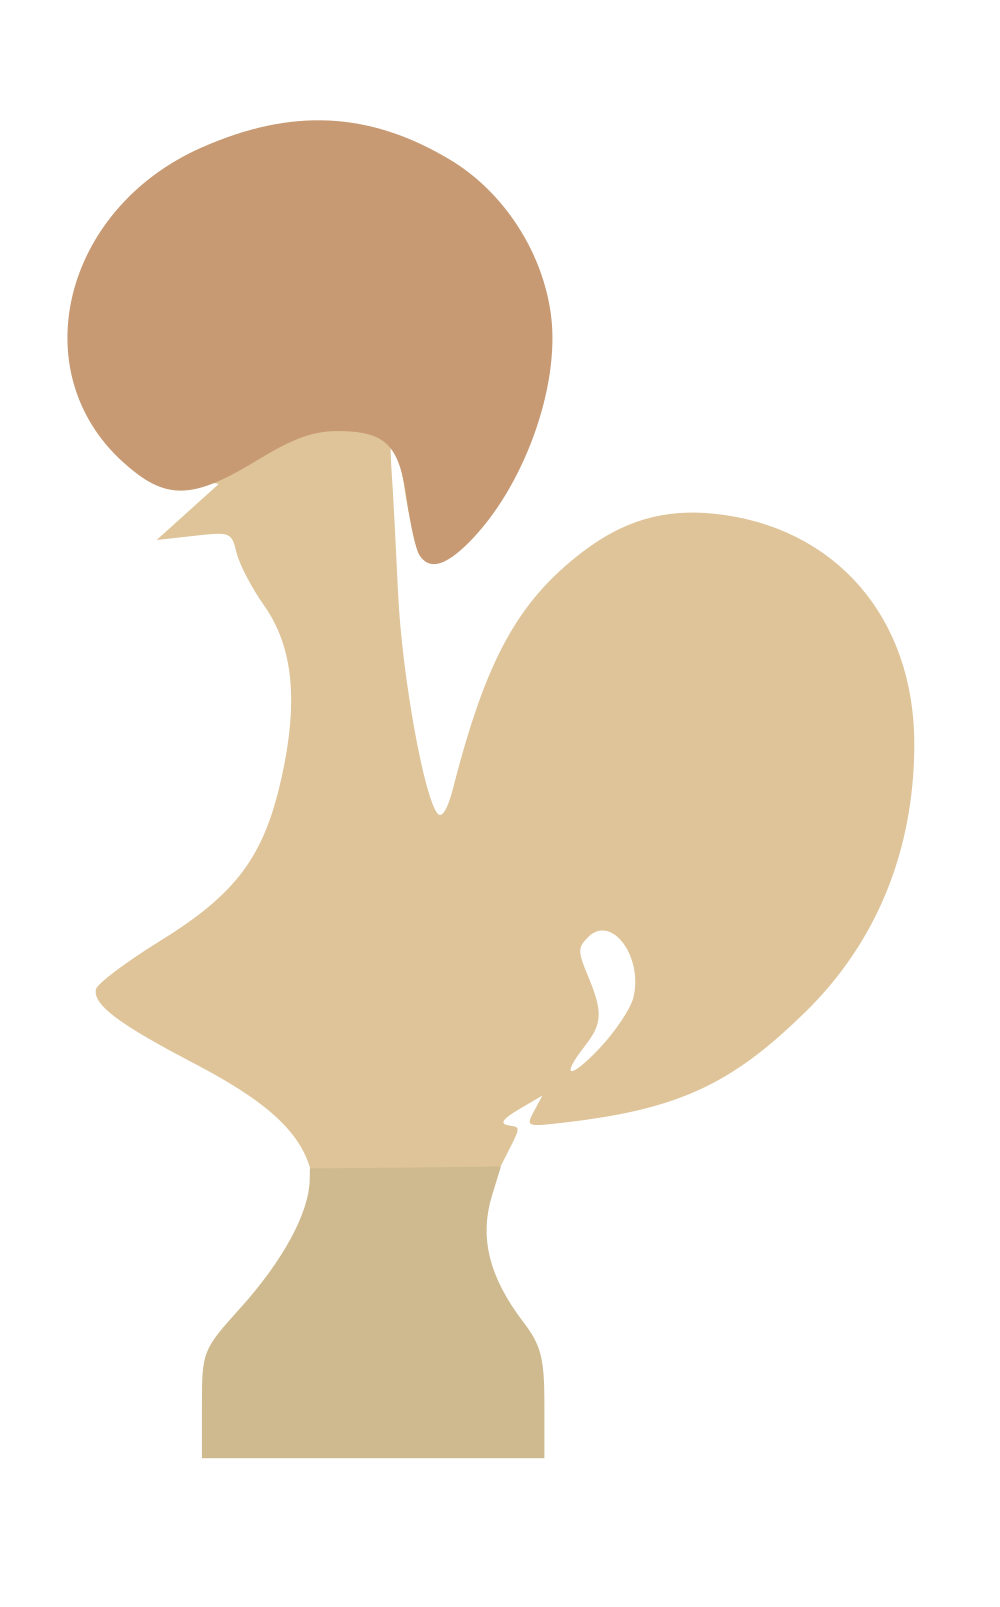
\includegraphics[width=0.15\textwidth]{coq-logo-large.png}
  \end{center}
\end{frame}

%%%%%%%%%%%%%%%%%%%%%%%%%%%%%%%%%%%%%%%%%%%%%%%%%%%%%%%%%%%%%%%%%%%%%%%

\end{document}
